\documentclass[a4paper,12pt,twoside,openany]{report}
%
% Wzorzec pracy dyplomowej
% J. Starzynski (jstar@iem.pw.edu.pl) na podstawie pracy dyplomowej
% mgr. inż. Błażeja Wincenciaka
% Wersja 0.1 - 8 października 2016
%
\usepackage{polski}
\usepackage{helvet}
\usepackage[T1]{fontenc}
\usepackage{anyfontsize}
\usepackage[utf8]{inputenc}
\usepackage[pdftex]{graphicx}
\usepackage{tabularx}
\usepackage{array}
\usepackage[polish]{babel}
\usepackage{subfigure}
\usepackage{amsfonts}
\usepackage{verbatim}
\usepackage{indentfirst}
\usepackage[pdftex]{hyperref}


% rozmaite polecenia pomocnicze
% gdzie rysunki?
\newcommand{\ImgPath}{.}

% oznaczenie rzeczy do zrobienia/poprawienia
\newcommand{\TODO}{\textbf{TODO}}


% wyroznienie slow kluczowych
\newcommand{\tech}{\texttt}

% na oprawe (1.0cm - 0.7cm)*2 = 0.6cm
% na oprawe (1.1cm - 0.7cm)*2 = 0.8cm
%  oddsidemargin lewy margines na nieparzystych stronach
% evensidemargin lewy margines na parzystych stronach
\def\oprawa{1.05cm}
\addtolength{\oddsidemargin}{\oprawa}
\addtolength{\evensidemargin}{-\oprawa}

% table span multirows
\usepackage{multirow}
\usepackage{enumitem}	% enumitem.pdf
\setlist{listparindent=\parindent, parsep=\parskip} % potrzebuje enumitem

%%%%%%%%%%%%%%% Dodatkowe Pakiety %%%%%%%%%%%%%%%%%
\usepackage{prmag2017}   % definiuje komendy opieku,nrindeksu, rodzaj pracy, ...


%%%%%%%%%%%%%%% Strona Tytułowa %%%%%%%%%%%%%%%%%
\title{Badanie algorytmów \linebreak[1]do~porównywania stylów tekstów w języku polskim}

% autor
\author{Szymon Masłowski}
\nrindeksu{271070}


\opiekun{dr inż. Grzegorz Sarwas}
\terminwykonania{12 Grudnia 2012} % data na oświadczeniu o samodzielności
\rok{2023}


% Podziekowanie - opcjonalne
\podziekowania{\noindent
{\Large Podziękowania}
\bigskip

Dziękujemy bardzo serdecznie wszystkim, a w szczególności Rodzinom i~Unii Europejskiej...

\bigskip

{\raggedleft
Zdolny Student i Pracowity Kolega

}

}

% To sa domyslne wartosci
% - mozna je zmienic, jesli praca jest pisana gdzie indziej niz w ZETiIS
% - mozna je wyrzucic jesli praca jest pisana w ZETiIS
%\miasto{Warszawa}
%\uczelnia{POLITECHNIKA WARSZAWSKA}
%\wydzial{WYDZIAŁ ELEKTRYCZNY}
%\instytut{INSTYTUT STEROWANIA\linebreak[1] I~ELEKTRONIKI PRZEMYSŁOWEJ}
% \zaklad{ZAKŁAD STEROWANIA}
%\kierunekstudiow{INFORMATYKA}

% domyslnie praca jest inzynierska, ale po odkomentowaniu ponizszej linii zrobi sie magisterska
%\pracamagisterska
%%% koniec od P.W

\opinie{%
  \newpage
\begin{center}
 {\large\bf  Opinia} \\
o pracy dyplomowej magisterskiej wykonanej przez dyplomanta\\
{\bf Zdolnego Studenta i Pracowitego Kolegę} \\
 Wydział Elektryczny, kierunek Informatyka,  Politechnika Warszawska\\
Temat pracy\\
\textit{\bf
TYTUŁ PRACY DYPLOMOWEJ
}\\
\end{center}
\medskip
\noindent
Promotor: {\bf dr inż. Miły Opiekun}\\
Ocena pracy dyplomowej: {\bf bardzo dobry}

\medskip

\centerline{\bf Treść opinii}
   Celem pracy dyplomowej panów dolnego Studenta i Pracowitego Kolegi  było
opracowanie systemu pozwalającego symulować  i opartego o oprogramowanie o
otwartych źródłach (ang. Open Source). Jak piszą Dyplomanci, starali się opracować
system, który łatwo będzie dostosować do zmieniających się dynamicznie wymagań,
będzie miał niewielkie wymagania sprzętowe i umożliwiał dalszą łatwą rozbudowę oraz
dostosowanie go do potrzeb.
Przedstawiona do recenzji praca składa się z krótkiego wstępu jasno i
wyczerpująco opisującego oraz uzasadniającego cel pracy, trzech rozdziałów (2-4)
zawierających opis istniejących podobnych
rozwiązań, komponentów rozpatrywanychjako kandydaci do
tworzonego systemu i wreszcie zagadnień wydajności wirtualnych
rozwiązań. Piąty rozdział to opis przygotowanego przez
Dyplomantów środowiska obejmujący opis konfiguracji
środowiska oraz przykładowe ćwiczenia laboratoryjne. Ostatni
rozdział pracy to opis możliwości dalszego
rozwoju projektu. W ramach przygotowania pracy Dyplomanci zebrali i przedstawili w
bardzo przejrzysty sposób duży zasób informacji, co świadczy o dobrej orientacji
w nowoczesnej i ciągle intensywnie rozwijanej tematyce stanowiącej
zakres pracy i o umiejętności przejrzystego przedstawienia tych
wyników. Praca zawiera dwa dodatki, z których pierwszy obejmuje wyniki
eksperymentów i badań nad wydajnością, a drugi to źródła
skryptów budujących środowisko.

 Dyplomanci dość
dobrze zrealizowali postawione przed nimi zadanie,
wykazali się więc umiejętnością zastosowania w praktyce wiedzy
przedstawionej w rozdziałach 2-4.  Uważam, że cele postawione w założeniach pracy zostały pomyślnie
zrealizowane. Proponuję ocenę bardzo dobrą (5).

\vskip 1cm
{
\raggedleft
(data, podpis)\kern1cm

}
  \newpage
  \newpage
\begin{center}
 {\large\bf  Recenzja } \\
pracy dyplomowej magisterskiej wykonanej przez dyplomanta\\
{\bf Szymona Masłowskiego} \\
 Wydział Elektryczny, kierunek Informatyka,  Politechnika Warszawska\\
Temat pracy\\
\textit{\bf
Badanie algorytmów \linebreak[1]do~porównywania stylów tekstów w języku polski
}\\
\end{center}
\medskip
\noindent
Recenzent: {\bf prof. nzw. dr hab. inż. Jan Surowy}\\
Ocena pracy dyplomowej: {\bf bardzo dobry}
\medskip


\centerline{\bf Treść recenzji}
   Celem pracy dyplomowej panów dolnego Studenta i Pracowitego Kolegi  było
opracowanie systemu pozwalającego symulować  i opartego o oprogramowanie o
otwartych źródłach (ang. Open Source). Jak piszą Dyplomanci, starali się opracować
system, który łatwo będzie dostosować do zmieniających się dynamicznie wymagań,
będzie miał niewielkie wymagania sprzętowe i umożliwiał dalszą łatwą rozbudowę oraz
dostosowanie go do potrzeb.
Przedstawiona do recenzji praca składa się z krótkiego wstępu jasno i
wyczerpująco opisującego oraz uzasadniającego cel pracy, trzech rozdziałów (2-4)
zawierających bardzo solidny i przejrzysty opis: istniejących podobnych
rozwiązań (rozdz. 2), komponentów rozpatrywanychjako kandydaci do
tworzonego systemu (rozdz. 3) i wreszcie zagadnień wydajności wirtualnych
rozwiązań, zwłaszcza w kontekście współpracy  kilku elementów
 sieci (rozdział 4). Piąty rozdział to opis przygotowanego przez
Dyplomantów środowiska obejmujący opis konfiguracji
środowiska oraz przykładowe ćwiczenia laboratoryjne (5 ćwiczeń). Ostatni, szósty
rozdział pracy to krótkie zakończenie, które wylicza także możliwości dalszego
rozwoju projektu. W ramach przygotowania pracy Dyplomanci zebrali i przedstawili w
bardzo przejrzysty sposób duży zasób informacji o narzędziach, Rozdziały 2, 3 i 4 świadczą o dobrej orientacji
w nowoczesnej i ciągle intensywnie rozwijanej tematyce stanowiącej
zakres pracy i o umiejętności syntetycznego, przejrzystego przedstawienia tych
wyników. Drobne  mankamenty tej części pracy to zbyt skrótowe omawianie
niektórych zagadnień technicznych, zakładające dużą początkową wiedzę czytelnika
i dość niestaranne podejście do powołań na źródła.
Utrudnia to w pewnym stopniu czytanie pracy i zmniejsza jej wartość dydaktyczną
(a ta zdaje się być jednym z celów Autorów), ale jest zrekompensowane zawartością
merytoryczną. Praca zawiera dwa dodatki, z których pierwszy obejmuje wyniki
eksperymentów i badań nad wydajnością, a drugi to źródła
skryptów budujących środowisko. Praca
zawiera niestety dość dużą liczbę drobnych błędów redakcyjnych, ale nie wpływają
one w sposób istotny na na jej czytelność i wartość. W całej pracy przewijają
się samodzielne, zdecydowane wnioski Autorów, które są wynikiem własnych i
oryginalnych badań.  Rozdział 5 i dodatki pracy przekonują mnie, że Dyplomanci dość
dobrze zrealizowali postawione przed nimi zadanie. Pozwala to stwierdzić, że
wykazali się więc także umiejętnością zastosowania w praktyce wiedzy
przedstawionej w rozdziałach 2-4. Kończący pracę rozdział szósty świadczy o
dużym (ale moim zdaniem uzasadnionym) poczuciu własnej wartości i jest
świadectwem własnego, oryginalnego spojrzenia na tematykę przedstawioną w pracy
dyplomowej. Uważam, że cele postawione w założeniach pracy zostały pomyślnie
zrealizowane. Proponuję ocenę bardzo dobrą (5).

\vskip 1cm
{
\raggedleft
(data, podpis)\kern1cm

}
}

\streszczenia{
  \newpage
\begin{center}
\large \bf
Badanie algorytmów \linebreak[1]do~porównywania stylów tekstów w języku polski
\end{center}

\section*{Streszczenie}
Praca składa się z krótkiego wstępu jasno i
wyczerpująco opisującego oraz uzasadniającego cel pracy, trzech rozdziałów (2-4)
zawierających opis istniejących podobnych
rozwiązań, komponentów rozpatrywanychjako kandydaci do
tworzonego systemu i wreszcie zagadnień wydajności wirtualnych
rozwiązań. Piąty rozdział to opis  środowiska obejmujący opis konfiguracji
środowiska oraz przykładowe ćwiczenia laboratoryjne. Ostatni
rozdział pracy to opis możliwości dalszego
rozwoju projektu. 
\TODO{Napisac to ^^}
\bigskip
{\noindent\bf Słowa kluczowe:} NLP, Klasyfikacja, Analiza stylu, Przetwarzanie języka naturalnego, eksploracja tekstu

\vskip 2cm

\TODO{ Przetłumaczyć to }
\begin{center}
\large \bf
THESIS TITLE
\end{center}

\section*{Abstract}
This thesis presents a novel way of using a novel algorithm to solve complex
problems of filter design. In the first chapter the fundamentals of filter design
are presented. The second chapter describes an original algorithm invented by the
authors. Is is based on evolution strategy, but uses an original method of filter
description similar to artificial neural network. In the third chapter the implementation
of the algorithm in C programming language is presented. The fifth chapter contains results
of tests which prove high efficiency and enormous accuracy of the program. Finally some
posibilities of further development of the invented algoriths are proposed.

\bigskip
{\noindent\bf Keywords:} thesis, LaTeX, quality

\vfill
}

\begin{document}
\maketitle

%-----------------
% Wstęp
%-----------------
\chapter{Wstęp}

Od kiedy człowiek zapisuje swoje myśli na świecie utrwalane jest coraz więcej danych. Pisane są listy, książki i krótkie wiadomości. Każdy z tych dzieł ma swojego autora, choć nie zawsze jest on znany. Niemniej dzięki uważnej obserwacji można ustalić kto jest autorem tekstu, jeżeli posiadamy inne do porównania. Pisanie, podobnie jak mowa czy każde działanie, które człowiek podejmuje, jest pod wpływem osobistego zachowania--stylu. Na podstawie sprawdzania stylu można przypisać autorstwo starożytnych tekstów, których autorzy mogli być zmieniani, bądź pominięci, albo odnaleźć autora anonimowego terrorystycznego manifestu. 
Celem tej pracy jest poruszenie tematu takiego automatycznego rozpoznawania tekstów, które napisane są w języku polskim. Tworzy to specyficzne warunki, w odróżnieniu od np. języka angielskiego. Chciałbym sprawdzić czy i z jaką pewnością można określić autora tekstu dodając go do zbioru kilku znanych autorów.

Opisać organizację pracy
\TODO powołać się na jakąś bibliografię


\chapter{Wprowadzenie do problematyki porównywania tekstów}

\section{NLP}
Pojęciem NLP (ang. Natural Language Processing) określa się zbiór technik komputerowych służących do analizy i reprezentacji tekstów występujących na poziomie analizy lingwistycznej w celu uzyskania sposobu przetwarzania języka przypominającego ludzki w określonym zakresie zadań i zastosowań. - Soldacki
\url{'https://pl.wikipedia.org/wiki/Przetwarzanie_języka_naturalnego'}
	
\section{Budowa zdania}
Tekst składa się ze znaków, tworzących słowa, składających się na zdania. Za Słownikiem Języka Polskiego, zdanie to 
\begin{enumerate}
	\item «myśl wyrażona słowami»
	\item "«zespół wyrazów powiązanych zależnościami gramatycznymi i zawierający orzeczenie»"
\end{enumerate}
\url{'https://encenc.pl/budowa-zdania/'}
\url{'https://pl.wikipedia.org/wiki/Szyk_wyrazów'}
\section{Klasyfikacja języków naturalnych}
\section{Styl tekstu}
Każdy człowiek jest inny, ze względu na swoje DNA, środowisko i temperament. To wszystko rzutuje na jego działania, zarówno rodzaj jak i sposób ich wykonania. Każda czynność, którą wykonuje człowiek obarczona podpisem wykonawcy, który jest mniej lub bardziej wyraźny. Niemniej czynności przez nas wykonywane są robione na nasz własny sposób. 
Tekst, który zapisujemy jest odbiciem naszego sposobu myślenia, więc rzutuje to na przykład na użyte słownictwo, czy sposób budowania zdań.
Cechy, które chcę użyć w pracy to:
\begin{itemize}
\item kolejność części mowy

Dzięki temu, że język polski jest językiem fleksyjnym, kolejność słów może ulegać znacznej zmianie, bez zmiany znaczenia zdania. Więc stała kolejność części zdania może być cechą charakterystyczną

\item zbiór słów - wektor binarny?

Ile różnych słów występuje, jak bogate słownictwo jest wykorzystywane. IDF do porównania jak bardzo różne od codziennego słownictwa jest to użyte w tekście.
\item złożoność zdań - ile takich zdań występuje? 

Czy zdania są proste, czy wielokrotnie złożone. Czy dzieje się to często, czy każde ze zdań jest takie.
\item Statystyka zdania/słów
	\begin{enumerate}
	\item Ile słów/zdanie 
	\item Jak długie słowa(znaki/sylaby)
	\item Ile słów krótkich <= 3 znaki
	\item Ile słów długich >= 7 znaków
	\item Monosylabowe słowa (1 sylaba)
	\item Wielosylabowe słowa (>= 3 sylaby)
	\item Najdłuższe zdanie (ilość słów)
	\item Najdłuższe słowo (ilość znaków, ilość sylab)
	\end{enumerate}
\item N-gramy literowe i słowne
N-gram jest ciągiem n elementów. Tworząc 2-gramy ze zdania \textit{Niezmiennik pętli jest techniką dowodzenia poprawności algorytmów.} Otrzymamy następujące 2-gramy:
\begin{itemize}
	\item Niezmiennik -- pętli
	\item pętli -- jest
	\item jest -- techniką
	\item etc.
W przypadku n-gramów literowych, zamiast słów używamy następujących po sobie liter. Ta cecha może mieć znaczenie w przypadku, kiedy autor ma jakieś problemy z wymową i naturalnie przez to nie będzie używał pewnego zakresu słów. 
\end{itemize}
\item (Odwrotna) Częstotliwość słów

Mówi nam o tym, jak szerokiego zasobu słów używa autor tekstu i w oparciu o korpus wzorcowy, jak ma się to do zwyczajów piśmienniczych danego czasu.
Odwrotna częstotliwość słów ( zwana dalej z ang. IDF --\textit{inversed document frequency }) 
\item Kwestia podstawowych form i przyrostów (archaizmy mają inne "rostki")
\item Indeksy czytelności tekstu

Te cechy są pośrednimi wskaźnikami, które będą ilościowym wyznacznikiem czy tekst jest "łatwy" czy "trudny" w odbiorze i czytaniu. 
	\begin{enumerate}
	\item SMOG
	
	\url{'https://en.wikipedia.org/wiki/SMOG'}
	\item Indeks czytelności Flescha-Kincaida
	
	\url{'https://en.wikipedia.org/wiki/Flesch-Kincaid_readability_tests'}
	\item Linsear Write
	
	\url{'https://en.wikipedia.org/wiki/Linsear_Write	'}
	\item Lix
	
	\url{'https://en.wikipedia.org/wiki/Lix_(readability_test)'}
	\end{enumerate}
\end{itemize} 	
	
	
\section{Analiza morfologiczna}
https://core.ac.uk/download/pdf/11337572.pdf - Bień
\section{Analiza syntaktyczna}
\url{'http://bazhum.muzhp.pl/media//files/Prace_Jezykoznawcze/Prace_Jezykoznawcze-r2008-t10/Prace_Jezykoznawcze-r2008-t10-s187-200/Prace_Jezykoznawcze-r2008-t10-s187-200.pdf'} ??
\section{Klasyfikacja}
In classification, inputs are divided into two or more classes, and the learner must produce a model that assigns unseen inputs to one or more (multi-label classification) of these classes. This is typically tackled in a supervised way. Spam filtering is an example of classification, where the inputs are email (or other) messages and the classes are "spam" and "not spam". - Richard O. Duda, Peter E. Hart, David G. Stork (2001) Pattern classification (2nd edition), Wiley, New York, ISBN 0-471-05669-3. Z wiki ^^

\chapter{Przegląd dostępnych rozwiązań}

\section{Rozprawa doktorska z EITI}
Napisał ziomek tekst i jest spoko.

\section{Jednolity System Antyplagiatowy}
Jednolity system antyplagiatowy jest w posiadaniu Ministra właściwego do spraw szkolnictwa wyższego, a jego budowa i administracja realizowana jest przez Ośrodek Przetwarzania Informacji - Państwowy Instytut Badawczy pod nadzorem Ministra właściwego do spraw szkolnictwa wyższego. System jest wymaganym elementem sprawdzającym czy praca dyplomowa jest samodzielna: jest plagiatem czy nie. 
Co ciekawe, autorzy przypominają na każdym kroku, że "Wynik badania antyplagiatowego nie stanowi ostatecznego rozstrzygnięcia czy praca dyplomowa jest plagiatem czy też nie.". 

\begin{figure}[!htbp]
	\begin{center}
		\centering
		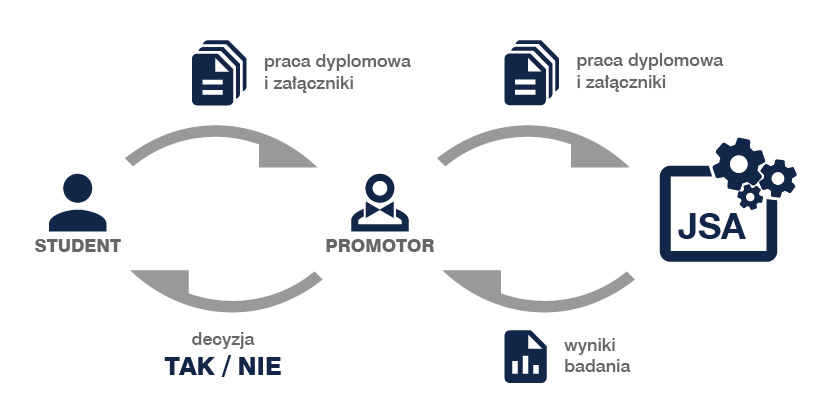
\includegraphics[scale=0.35]{\ImgPath/rys/jsa_infograf-01.jpg}
	\end{center}
	\caption{Infografika pokazująca proces użycia JSA}
\end{figure}

System generuje wynik na podstawie płaszczyzn i cech prezentowanych w grupach wg obszarów, których dotyczą: 
\begin{itemize}
	\item \textbf{Analiza tekstu} jest pierwszym obszarem sprawdzenia pracy. Polega głównie na sprawdzeniu czy w tekście nie pojawiają się białe znaki i nie zostały wykorzystane inne techniki, mające na celu zaburzyć automatyczne przetworzenie tekstu i jednoczesnej neutralności dla ludzkiego czytelnika. \linebreak 
	Na te techniki składają się znaki białe, bądź pochodzące z innego języka a graficznie będące podobne do języka pracy. Te techniki zmieniają długości słów, przez co porównania do innych "czystych" tekstów są nieefektywne. Na podstawie porównania rozkładu długości i częstości słów z danymi z Ogólnopolskiego Repozytorium Pisemnych Prac Dyplomowych można znajdować przesłanki, że nastąpiły takie manipulacje. \linebreak
	Dodatkowo System bada spójność ogólnopojętego stylu tekstu i oczekuje, że co najmniej 70\% tekstu będzie napisana w takim samym stylu. Niestety nie jest udostępnione na jakiej podstawie badany jest styl.
	  
	\item \textbf{Procentowy Rozmiar Podobieństwa} jest wskaźnikiem, który pokazuje jak duża część pracy składa się z fragmentów pochodzących z innych tekstów. Proponowane są 4 rozmiary zbiorów porównawczych: dla ciągów słownych nie dłuższych niż 5, 10, 20 i 40 słów. Dodatkowo tworzona jest lista źródeł (w przypadku, gdy fragment zostanie gdzieś odnaleziony).
	
\end{itemize}


\section{Otwarty System Antyplagiatowy}


\section{Bank ING i czytelność dokumentóW}
\section{Użyte technologie}
\subsection{Python}
\subsection{Biblioteki}

\chapter{Model klasyfikacji}
\section{Warunki}
\subsection{Ile użytych tekstów/autorów}
\section{Metody porównywania obiektów}
\subsection{SVM}

\section{Budowa i opis algorytmu}
\subsection{Przygotowanie danych}
\subsection{Struktura danych}
\subsection{Cechy}
\subsection{Algorytmy użyte do ekstrakcji cech}
\subsection{Klasyfikacja}

\chapter{Testy i wyniki}
\section{Przypadki testowe}
\section{Cel testów}
\section{Wyniki}

\chapter{Wyniki}
\section{Czy było warto?}
\section{Podjęte decyzje}
\subsubsection{Klasyfikator}
Do rozwiązania zagadnienia klasyfikacji można użyć wielu rozwiązań, takich jak: sieci neuronowe, klasyfikator Bayesowski, drzewo decyzyjne, metoda najbliższych sąsiadów czy w końcu SVM. Ze względu na rozmiar pracy, postanowiłem nie sprawdzać wpływu różnych klasyfikatorów na dokładność wyniku. Jak pokazują inne prace, użycie tego klasyfikatora zapewniało najdokładniejsze wyniki.

\TODO {bibliografia wyliczenia}

\TODO {bibliografia, że SVM jest ok do tekstów}

\subsubsection{Kolejna decyzja}

\section{Co należało by poprawić?}



\appendix
\chapter{Pierwszy dodatek} 

\begin{thebibliography}{99}
\addcontentsline{toc}{chapter}{Bibliografia}
\bibitem{Stevens}{W. R. Stevens, G. R. Wright, ,,Biblia TCP/IP tom 1'', RM, 
1998.}

\end{thebibliography}

\zakonczenie  % wklejenie recenzji i opinii

\end{document}
%+++ END +++
